\documentclass[border=6pt]{standalone}
\usepackage{amsmath}
\usepackage{tikz}
\usetikzlibrary{arrows.meta}
\begin{document}
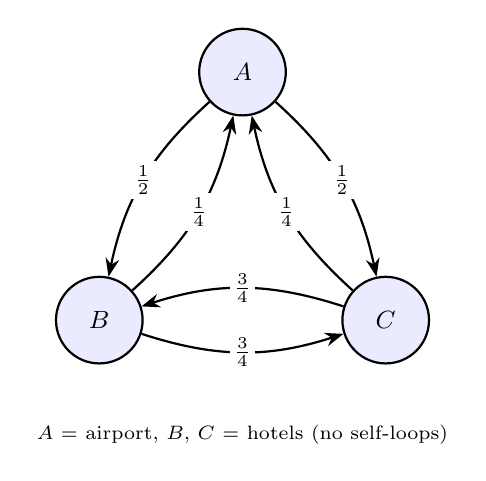
\begin{tikzpicture}[>=Stealth,font=\small,
 s/.style={draw,thick,circle,minimum size=1.1cm,inner sep=0pt,fill=blue!8},
 e/.style={->,thick},
 lab/.style={font=\small,fill=white,inner sep=1.5pt},
 every loop/.style={->,thick,looseness=6}]
\node[s] (A) at (90:2.1) {$A$};
\node[s] (B) at (210:2.1) {$B$};
\node[s] (C) at (-30:2.1) {$C$};
\draw[e] (A) to[bend right=18] node[lab]{$\tfrac12$} (B);
\draw[e] (B) to[bend right=18] node[lab]{$\tfrac14$} (A);
\draw[e] (A) to[bend left=18] node[lab]{$\tfrac12$} (C);
\draw[e] (C) to[bend left=18] node[lab]{$\tfrac14$} (A);
\draw[e] (B) to[bend right=18] node[lab]{$\tfrac34$} (C);
\draw[e] (C) to[bend right=18] node[lab]{$\tfrac34$} (B);
\node[font=\scriptsize,align=center] at (0,-2.5) {$A$ = airport, $B$, $C$ = hotels (no self-loops)};
\end{tikzpicture}
\end{document}
